\section{Resoconto delle attività di verifica}
In seguito vengono presentati i resoconti delle attività di verifica svolte.
Questa sezione viene mantenuta in costante aggiornamento rispetto alle revisioni di avanzamento del progetto.
\subsection{Revisione dei Requisiti}
\subsubsection{Analisi statica dei documenti}
L'analisi statica dei documenti ha portato alla produzione di una lista degli errori comuni. Questa lista, che deve essere mantenuta aggiornata con le prossime analisi, andrà a facilitare il compito dei verificatori.
\subsubsection{Esiti delle verifiche} 
\paragraph{Indice di Gulpease}\mbox{} %mbox perché altrimenti il paragraph finisce sotto al contenuto
%\subparagraph{Revisione dei Requisiti} \mbox{}
\begin{longtable} {						
		>{}p{50mm}  		
		>{}p{8mm}		
		>{}p{8mm}		
		>{}p{8mm}		
		>{}p{8mm}		
		>{}p{8mm}		
		>{}p{8mm}
		>{}p{8mm}
		>{}p{8mm}
		>{}p{8mm}				
	}			
	\rowcolor{gray!50}
	\textbf{Documento} & \textbf{I} & \textbf{II} & \textbf{III} & \textbf{IV} & \textbf{V} & \textbf{VI} \TBstrut \\ [2mm]
	\textbf{Analisi dei Requisiti} & - & - & - & - & - & - \TBstrut \\ [2mm]
	\textbf{Studio di Fattibilità} & 95 & 94 & 98 & 97 & 96 & 100 \TBstrut \\ [2mm]
	\textbf{Norme di Progetto} & 43 & 54 & 57 & 58 & 60 & 63 \TBstrut \\ [2mm]
	\textbf{Piano di Progetto} & - & - & - & - & - & - \TBstrut \\ [2mm]
	\textbf{Piano di Qualifica} & - & - & - & - & - & - \TBstrut \\ [2mm]
	\textbf{Glossario} & - & - & - & - & - & - \TBstrut \\ [2mm]
	\textbf{Verbali interni (media)} & 87 & 85 & 84 & 83 & 81 & 78 \TBstrut \\ [2mm]
	\textbf{Verbali esterni (media)} & - & - & 62 & 62 & 61 & 61 \TBstrut \\ [2mm]
	\rowcolor{white}
	\caption{Indice di Gulpease Revisione dei Requisiti}
\end{longtable}
\begin{figure}[H] 	
	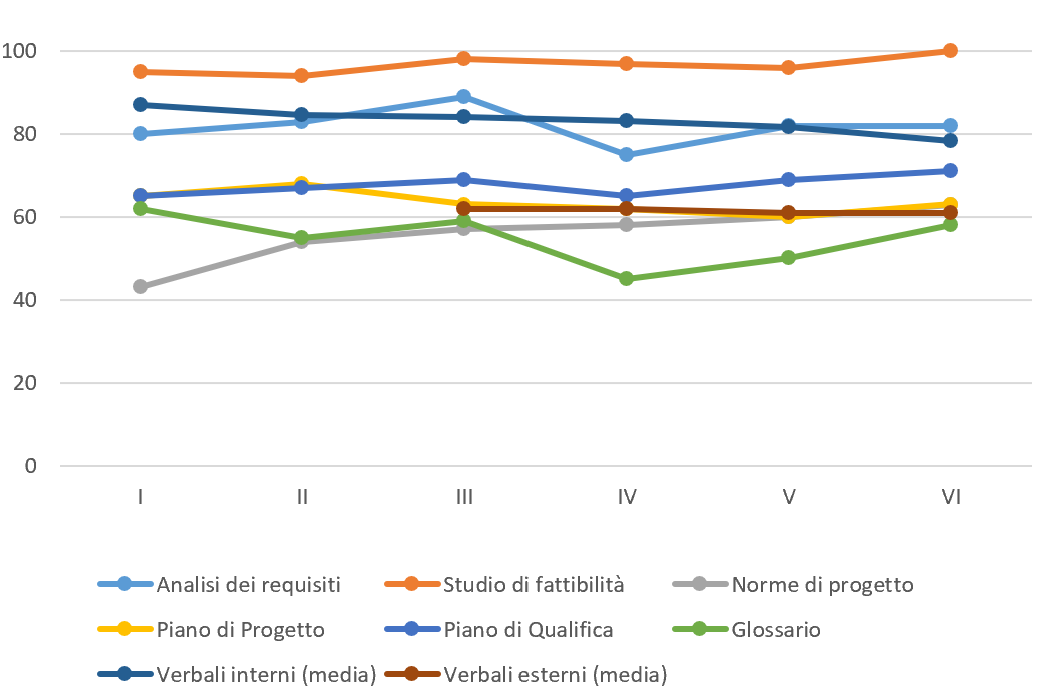
\includegraphics[width=\linewidth]{./img/grafici/2.png}	
	\caption{Indice di Gulpease Revisione dei Requisiti}	
\end{figure}

\begin{longtable} {						
		>{}p{50mm}  		
		>{}p{8mm}		
		>{}p{8mm}		
		>{}p{8mm}		
		>{}p{8mm}		
		>{}p{8mm}		
		>{}p{8mm}
		>{}p{8mm}				
	}			
	\rowcolor{gray!50}
	\textbf{Documento} & \textbf{RR} & \textbf{RP} & \textbf{RQ} & \textbf{RA} \TBstrut \\ [2mm]
	\textbf{Analisi dei Requisiti} & - & - & - & - \TBstrut \\ [2mm]
	\textbf{Studio di Fattibilità} & 100 & - & - & - \TBstrut \\ [2mm]
	\textbf{Norme di Progetto} & 63 & - & - & - \TBstrut \\ [2mm]
	\textbf{Piano di Progetto} & - & - & - & - \TBstrut \\ [2mm]
	\textbf{Piano di Qualifica} & - & - & - & - \TBstrut \\ [2mm]
	\textbf{Glossario} & - & - & - & - \TBstrut \\ [2mm]
	\textbf{Verbali interni (media)} & 78 & - & - & - \TBstrut \\ [2mm]
	\textbf{Verbali esterni (media)}& 61 & - & - & - \TBstrut \\ [2mm]
	\rowcolor{white}
	\caption{Indice di Gulpease}
\end{longtable}
\begin{figure}[H] 	
	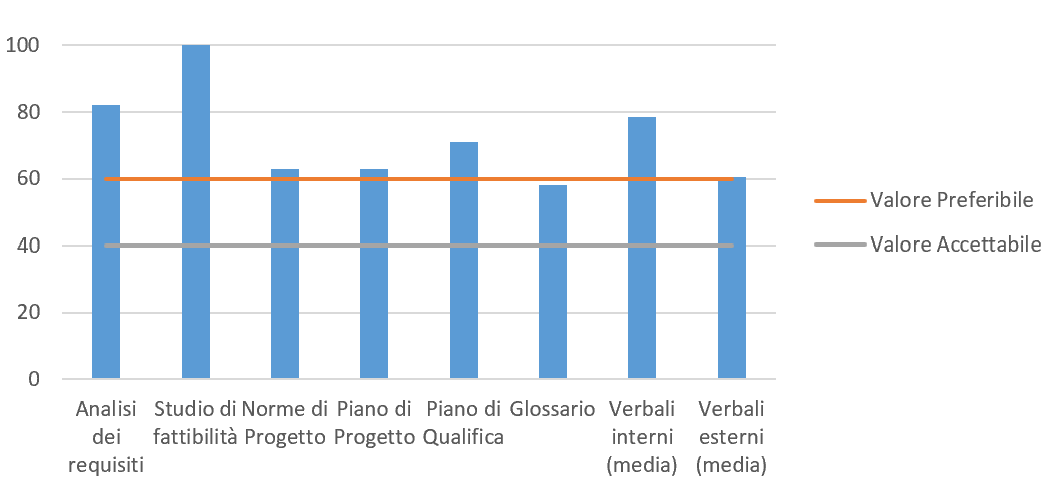
\includegraphics[width=\linewidth]{./img/grafici/1.png}	
	\caption{Indice di Gulpease}	
\end{figure}